\documentclass{sig-alternate-05-2015}

\usepackage{amsmath}

\begin{document}

\title{YoloFlow}

\numberofauthors{3}
\author{
\alignauthor
Konstantine Buhler\\
       \email{buhler@stanford.edu}
\alignauthor
John Lambert\\
       \email{johnwl@stanford.edu}
\alignauthor
Matthew Vilim\\
       \email{mvilim@stanford.edu}
}
\maketitle
\begin{abstract}
Todo
\end{abstract}

\section{Introduction}
Todo

\section{Overview}
\subsection{Basics of YOLO}

\subsection{Motivation}

\section{TensorFlow Implementation}
YOLO is implemented as a 32 layer deep convolutional neural network (DNN). The open source implementation released along with the paper is built upon a custom DNN framework called \textit{darknet} \footnote{github.com/pjreddie/darknet}. This application provides the baseline by which we compare our implementation of YOLO. Redmon et al. have released several variants of YOLO. For our purposes, we chose the variant outlined in \cite{redmon:yolo}. In places in which the paper lacks details, we refer to the baseline \textit{darknet} implementation to resolve ambiguities.

The TensorFlow implementation was performed in two stages. First, we constructed the dataflow graph, importing pre-trained weights from \textit{darknet}. With the pre-trained dataset, inference may be performed easily without need to create the loss function used during training. Our dataflow graph implementation is shown in Figure [TODO]. This graphical representation of the model was generated by TensorBoard, an included profiling tool that can be used to understand and visualize TensorFlow's execution.

\subsection{Weight conversion}
To simplify the port of YOLO from \textit{darknet} to TensorFlow, we begin by using a pre-trained model. This greatly simplifies debugging as we can obtain immediate results from our execution without the need to implement a loss function and back propogation to adjust the weights. Furthermore, training a new model is naturally slow. For example, our pre-trained model was trained by \cite{redmon:yolo} for a week on the latest high-performance GPUs.

However, choosing a pre-trained model is disadvantageous in that we must interface with a data format chosen by the model's author. In this case, we select one of YOLO's pre-trained models, \textit{yolo\_small.weights} provided on the author's website \footnote{pjreddie.com/darknet/yolo/}. These weights are represented as a large binary blob of 32 bit floating points for each layer's weight/bias values. We modify the source of \textit{darknet} to export the weights in a portable machine-independent format convenient for use in TensorFlow, comma-separated values (CSV). Parsing these large weight files (approximately 1GB) takes several minutes, so after they have been initialized in TensorFlow, we save a compressed TensorFlow \textit{.ckpt} file for quick reload (available for download our project's Github page).

\subsection{Model validation}
As the original YOLO paper serves only a summary of YOLO, it omits many details. Details of the 2D convolution parameters and connection between convolutional and fully connected layers were taken from the \textit{darknet} implementation. Validation and debug is drastically simplified in comparison to developing a new neural network model. Each input and output of our model can be compared with that of the \textit{darknet} implementation to ensure correctness or discover bugs. For example, during development the weights were being read in an improper sequence at a particular convolutional layer. Comparing the output of the two network's allowed the problem to quickly narrowed down and corrected.

For this checkpoint, we have validated the outputs of both networks match on the pre-trained model for the test image shown in Figure \ref{fig:test_image}. However, we have yet to parse the prediction output in order to calculate and draw bounding boxes. As in \textit{darknet}, the inputs are processed and resized with OpenCV to be $(448, 448)$ with three normalized color channels.

\begin{figure}
\centering
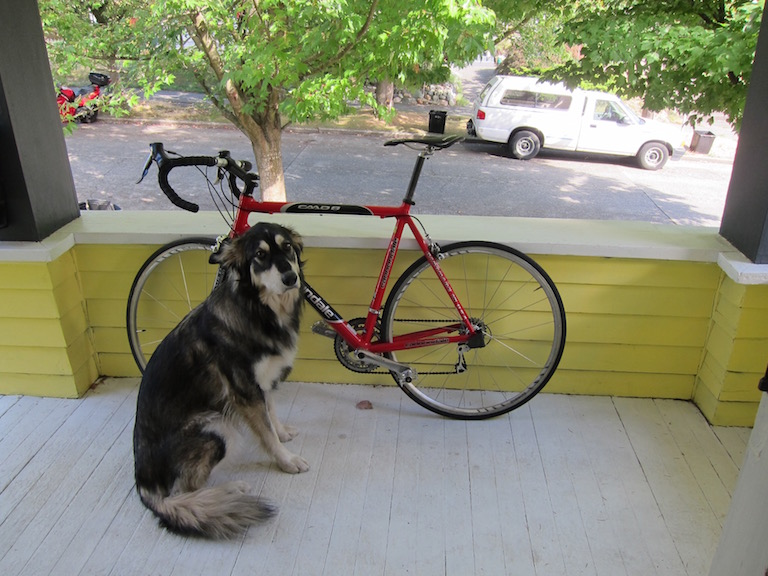
\includegraphics[width=\linewidth]{../data/dog.jpg}
\caption{Test image}
\label{fig:test_image}
\end{figure}

\bibliographystyle{abbrv}
\bibliography{yoloflow}

\end{document}
